\chapter{Related Work}

\label{ch:related_work}

%123456789 123456789 123456789 123456789 123456789 123456789 123456789 123456789

Great advantages offered by the usable re-identification algorithm also bring a considerable amount of research in the area. In this chapter, we aim to review this research and related articles. Furthermore, we also focus on the popular architectures of \glspl{nn} for image processing (not necessarily targetted for \reid{}).


\section{Person \Reid{}}

\label{sec:person_reid}

The problem of \reid{} has been an active research area for the past few decades and still is today. Many different approaches were explored by this date. Most of the designs embed the input image of the person into a specific feature space. Resulting feature vectors are then compared using some standard distance function. In combination with a suitably selected threshold, this produces the desired answer whether there is the same person on selected images or not (\cite{cheng2016person}). However, even designs that seek to directly answer the question without embedding the images into some intermediate feature space were explored (\cite{li2014deepreid}).

\subsection{Early Research}
\label{sec:early_research}

Many early attempts in tracking and re-identification describe the images using colors and color histograms in particular. For example, work presented by \cite{krumm2000multi} shows the usage of color histograms to perform tracking in the indoor environment.

Another interesting research was shown by \cite{orwell1999multi}. Again the authors extract color histograms. These histograms are then matched to identities by using \gls{em} over a set of Gaussians.

Even though the use of color histograms was later somewhat overshadowed by more complex techniques such as deep learning, some researchers still use it to perform \reid{}. For example, \cite{zeng2014person} combines the color histogram with spatial information to obtain better results.

Aside from the color histograms, we can see a variety of new techniques emerging. A technique based on the principal axes is presented by \cite{hu2006principal}. Ability to correctly identify the axes heavily relies on successful filtering out the background. The filtering is especially challenging in the scenarios where the occlusion is present or if people move in crowds. The authors propose a special version of the approach to tackle these challenging scenarios. Once the silhouette of a person is established, the principal axis is found. The algorithm then infers the position of the ``ground-point'', i.e., the point where the person touches the ground (this is usually the point where the principal axis intersects the lower bound of the bounding box but it may not be so simple in the case of occlusion). Based on these ``ground-points`` with the use of the Kalman filter, the algorithm then tracks the people. In order to re-identify the person across multiple cameras, the homography is firstly computed using suitable landmarks. Based on this obtained homography, it is straight-forward to compute the sets of points in each camera's view corresponding to the same ``ground-point''. A simple algorithm for maximum likelihood is used to establish a suitable matching (\reid{}) of detected people.

\subsection{Era of the Deep Neural Networks}

More and more successful models based on the deep learning emerged in the past few years. As well as many other image processing task, this field also came to a new era of proposed approches based on \glspl{nn}.

One such research is presented by \cite{ding2015deep}. The authors propose a relatively simple \gls{nn} consisting only of a few convolutional layers, interwoven with the max-pooling layers. To train the network, they use a Triplet Loss (albeit using non-standard terminology). They elaborate more on the selection of the triplets to train on.

A similar approach was explored by \cite{cheng2016person}. The basis of their method is again convolutional \gls{nn} trained by Triplet Loss. However, they presented several notable improvements. Firstly, the architecture they designed after the first convolutional layer ``splits'' the input into four horizontal strips. Meaning that each of these strips is fed into its own independent part of the \gls{nn}, where each part tries to learn the features of its respective body part. However, the original information is also used (``copied'') into the fifth ``global'' part of the \gls{nn} and trained. At the end of the \gls{nn} pipe-line, the parts' outputs are combined. The loss function used is again the Triplet Loss. The authors also focused on the formulation of Triplet Loss. They propose a slightly different formulation of the Triplet Loss, designed specifically for the \reid{} task.

Another \gls{nn} design is presented by \cite{li2014deepreid}. Unlike other approaches, they do not use Triplet Loss or a similar loss to embed the original images into feature space. The architecture they propose directly processes pair of images. The output of the whole network is then simply a number which describes ``confidence'' of the \gls{nn} how likely the images display the same person. Such architecture is then trained via simple softmax loss.

Additional work that tries to solve this problem with the usage of deep \gls{nn} is presented by \cite{hermans2017defense}. They experiment with the hand-crafted architecture of the neural network, as well as the pre-trained ResNet model, (we review ResNet in \autoref{ssec:resnet}). They further elaborate on the topic of Triplet Loss and suitable triplet selection.

Quite elaborate deep network architecture is offered by \cite{xu2018attention}. Their Attention-Aware Compositional Network can be broken into several parts. Firstly, the network tries to estimate an attention map and a visibility score for each body part (given body parts are setup by researchers prior learning). Based on the visibility, the features are extracted for the given parts. Finally, the feature vector representing the original image is produced by selected base network.

\section{Image Processing Architectures}

\label{sec:existing_architectures}

In this section, we further review a few very popular \gls{nn} architectures for image processing. Even though they are not specifically designed for re-identification, we utilize both their architectures and the weights trained for classification tasks that we use via means of the transfer learning (see \autoref{ssec:transfer_learning}).

We present more in detail two well-known \gls{nn} -- MobileNet and ResNet. Both of them presented a break-through in their own category at the time they were introduced.

\subsection{Residual Networks}
\label{ssec:resnet}


Residual networks (commonly referred to as just ResNets) are a quite popular family of \gls{nn} architectures designed especially for processing images. The first ResNet was officially introduced and described by \cite{resnet} and later improved by \cite{resnetimp}. With this model the authors won a few image processing competitions and as such the architecture immediately became very popular. The model won the first places at ILSVRC competition on the tasks of ImageNet detection, ImageNet localization (\cite{imagenetresults}) as well as COCO detection and COCO segmentation at COCO competition (\cite{cocodataset}). To this date this architecture remains inspiration for various state-of-the-art models and approaches.

Next, we investigate the proposed ResNet architecture and the motivations behind it. The authors tried to solve the problem of low training accuracy of the deep neural networks compared to their shallower counterparts. This counter-intuitive phenomenon led them to the following design change.

For a given layer, instead of learning direct suitable mapping $H(\vec{x})$, they designed the layer to learn just the ``residuum'' $H(\vec{x}) - \vec{x} = F(\vec{x})$ (hence the name). This was achieved by adding a residual connection between layer $n$ and layer $m > n$. The output of layer $n$ and layer $m - 1$ would be added together (see \autoref{fig:resnet_schema}), effectively pushing the layer $m$ to learn the residuum with respect to the output of layer $n$ rather than the whole original function.

\begin{figure}
    \centering
    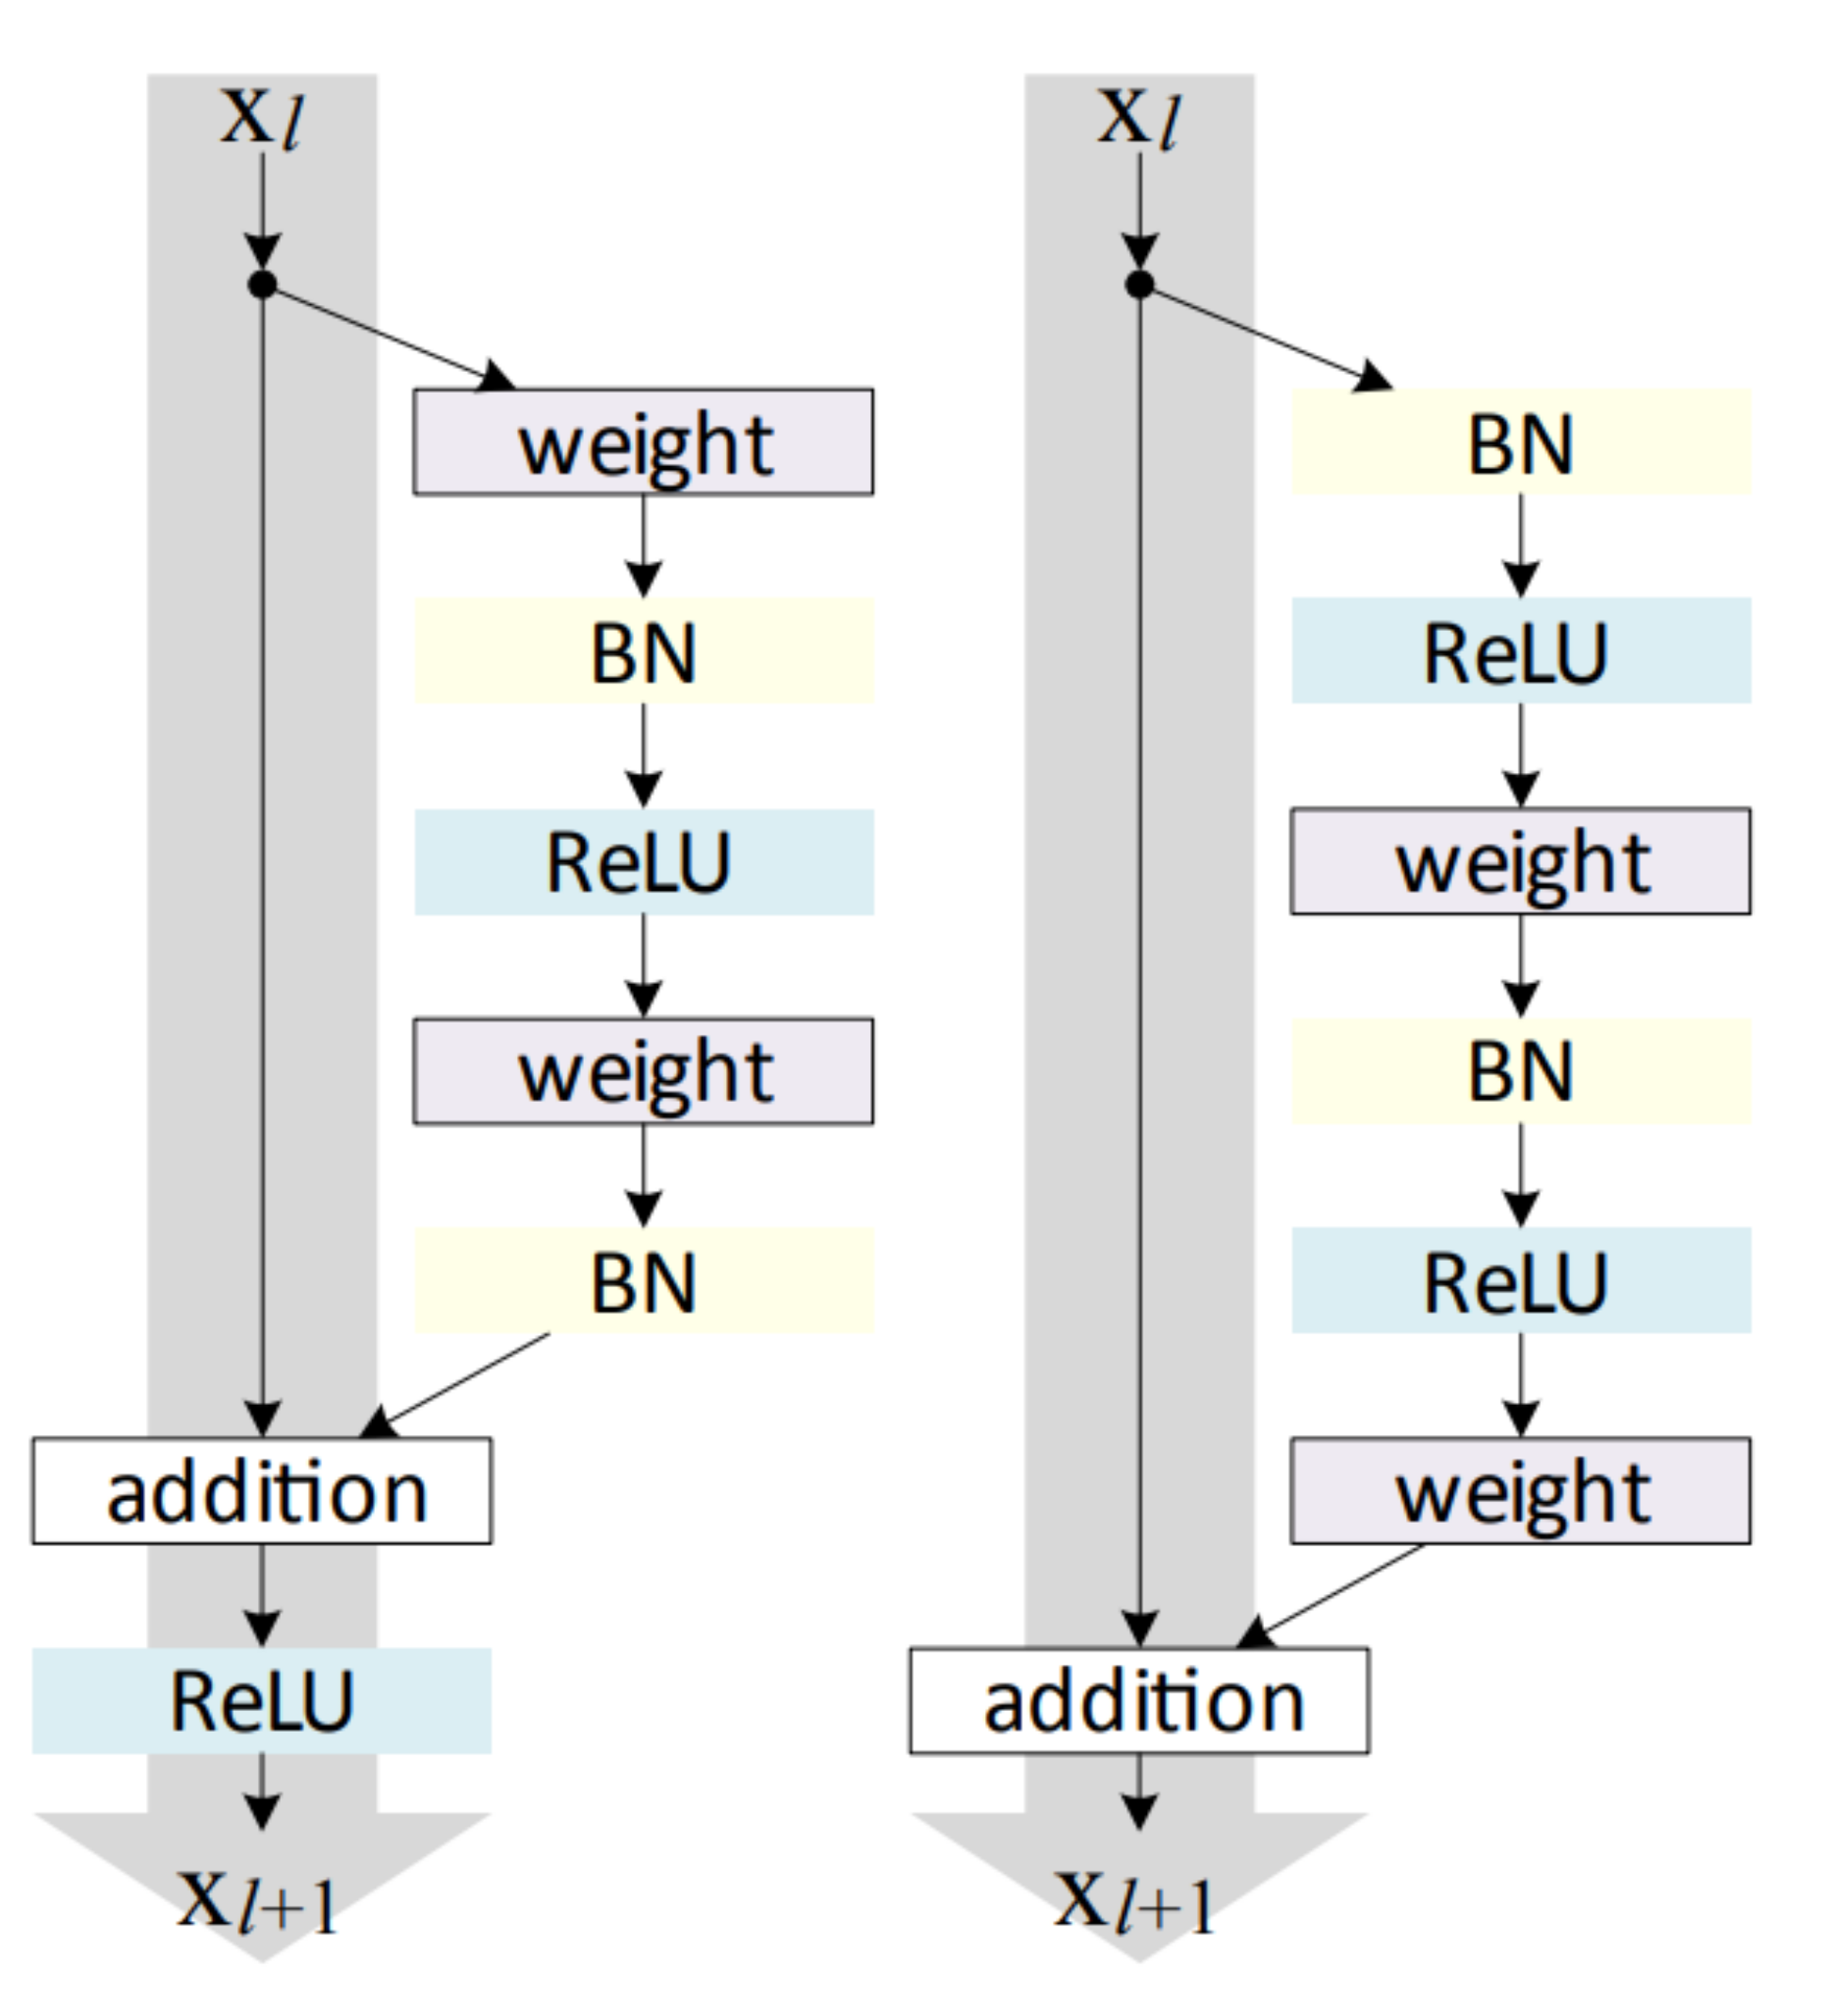
\includegraphics[width=0.48\textwidth]{img/resnetv2.png}
    \caption[Residual units]{Schema of the ``residual units''. On the left as presented by \cite{resnet}. The improved version by \cite{resnetimp} is on the right. Source: \cite{resnetimp}}
    \label{fig:resnet_schema}
\end{figure}

The rationale behind this change is that by adding layers that perform identity function, we can not worsen (or change at all for that matter) the network's output. Therefore, if we take a shallow network and increase its complexity by adding new layers, the (training) error should not decrease if the learning to approximate identity function is easily achieved. However, as the training error increases in traditional design, it can be argued that learning identity function is quite hard using gradient descent algorithm. By adding the residual connection, the problem of learning to approximate identity function becomes just a task of driving the weights of the connections to zero, which should be easier than to learn the identity function directly. As already mentioned, this rationale was successfully empirically proved on several tasks.

The original authors further improved this design in \cite{resnetimp} by reorganizing the layers in the network. They removed the activation function from the residual connection (or, more precisely, they moved it to the ``skipped'' part of the \gls{nn}). This way, they simplified the shortcut even more (see \autoref{fig:resnet_schema}). They further support this change by thorough empirical testing. Since then the ResNets and their derivates became an iconic break-though in deep learning.

\subsection{MobileNets}

\label{ssec:mobilenet}

Other notable architectures are MobileNets by \cite{mobilenets}. In these architectures, authors successfully created models with relatively low latency while maintaining a high accuracy level. The motivation behind such architecture is to provide suitable models for usage in mobile vision applications. They achieved the lowered latency of inference by simplifying some operations in the \gls{nn}.

The most notable change is the replacement of the standard convolutional layers as described in \autoref{sec:conv} by a pair of layers -- depthwise convolutional filter and pointwise convolutional filter.

In the first of these layers -- depthwise convolutional filter -- the convolution is applied on each input channel separately:

$$y_{i, j, r} = \sum_{k, l} x_{i+k, j+l, r} \, c_{k, l, r}$$
The latter of these two layers -- pointwise convolution filter -- is just simple convolution with kernel of size $1 \times 1$.

This replacement of the convolutional layer by two simpler layers significantly decreases the computation cost of inference and the time required for training such a network. The high accuracy of the resulting \glspl{nn} was empirically verified on the ImageNet tasks.

This architecture was then further improved by \cite{mobilenetv2} by introducing inverted residuals and linear bottlenecks. As these concepts are quite complex, we refer the reader to the original article for more information.


\section{Object Detection}

In this thesis, we focus on actual \reid{} within the stream. Prior to the \reid{} the object must be located within the stream itself. For this purpose, we use a third-party neural network. In particular, we use the network designed by \cite{dobransky2019}. The network is based on the Single Shot Detector (\cite{liu2016ssd}) adjusted to the ResNet architecture for low latency to allow real-time video stream processing. As object detection is not a topic of our work, we shall refer the reader to the original work for more details.

